\documentclass[aspectratio=169,10pt]{beamer}

% Theme selection
\usetheme{Madrid}
\usecolortheme{whale}

% Remove navigation symbols
\setbeamertemplate{navigation symbols}{}

% Packages
\usepackage[utf8]{inputenc}
\usepackage{amsmath,amssymb,amsfonts}
\usepackage{graphicx}
\usepackage{booktabs}

% Title, Author, and Course Information
\title[Traffic Flow ODE Modeling]{Traffic Flow Modeling and Prediction Using Nonlinear Ordinary Differential Equations}
\subtitle{Scientific Computation Project}
\author[Saba Dumbadze]{Saba Dumbadze}
\institute[KIU]{Scientific Computation \\ Kutaisi International University}
\date{23 October 2026}

\begin{document}

% =============================================================================
% SLIDE 1: Title Slide
% =============================================================================
\begin{frame}
  \titlepage
\end{frame}

% =============================================================================
% SLIDE 2: Problem Formulation and the Initial Value Problem
% =============================================================================
\begin{frame}{Problem Formulation and the Initial Value Problem}
  \begin{block}{The Initial Value Problem (IVP)}
    Find $y : [a, b] \to \mathbb{R}^n$ satisfying:
    \[
      y'(t) = f(t, y(t)), \quad y(a) = y_a
    \]
  \end{block}

  \begin{itemize}
    \item \textbf{Time grid}: Divide $[a, b]$ into $m$ intervals of step size $h = (b-a)/m$:
    \[
      t_n = a + n h, \quad n = 0, 1, \dots, m
    \]
    \item \textbf{Goal}: Compute numbers $y_n \approx y(t_n)$ that approximate the true continuous traffic flow.
    \item \textbf{Application}: Highway traffic flow across consecutive highway segments over time.
  \end{itemize}
\end{frame}

% =============================================================================
% SLIDE 3: Highway Traffic Flow ODE Model
% =============================================================================
\begin{frame}{Highway Traffic Flow ODE Model}
  \begin{block}{Conservation of Vehicles (System of 3 Coupled ODEs)}
    For each road segment $i \in \{1, 2, 3\}$, the vehicle count changes by inflow minus outflow:
    \[
      \frac{d x_i}{dt} = q_{\text{in}, i}(t) - q_{\text{out}, i}(t, x_i)
    \]
  \end{block}

  \begin{itemize}
    \item \textbf{State variables}: $x_1(t), x_2(t), x_3(t)$ are traffic volumes on segments 1, 2, and 3.
    \item \textbf{Input flow}: Segment 1 receives external upstream flow $u(t)$ from highway sensors.
    \item \textbf{Coupling}: Outflow from segment 1 feeds directly into segment 2, and segment 2 feeds into segment 3.
    \item \textbf{Nonlinear outflow}: Flow slows down at higher densities:
    \[
      q_{\text{out}, i} = \alpha_i x_i + \beta_i x_i^2
    \]
    where $\alpha_i, \beta_i > 0$ are physical highway parameters.
  \end{itemize}
\end{frame}

% =============================================================================
% SLIDE 4: Euler Schemes: Explicit and Implicit
% =============================================================================
\begin{frame}{Euler Schemes: Explicit and Implicit}
  \begin{columns}[onlytextwidth,T]
    \begin{column}{0.48\textwidth}
      \begin{block}{Explicit (Forward) Euler}
        \[
          y_{n+1} = y_n + h f(t_n, y_n)
        \]
        \begin{itemize}
          \item Derived from forward difference:
          \[
            \frac{y(t_{n+1}) - y(t_n)}{h} \approx y'(t_n)
          \]
          \item Direct calculation: only requires one evaluation of $f$ per step.
          \item Simple and very fast to compute.
        \end{itemize}
      \end{block}
    \end{column}

    \begin{column}{0.48\textwidth}
      \begin{block}{Implicit (Backward) Euler}
        \[
          y_{n+1} = y_n + h f(t_{n+1}, y_{n+1})
        \]
        \begin{itemize}
          \item Derived from backward difference:
          \[
            \frac{y(t_{n+1}) - y(t_n)}{h} \approx y'(t_{n+1})
          \]
          \item The unknown $y_{n+1}$ appears on both sides.
          \item Requires solving an algebraic equation at every step.
        \end{itemize}
      \end{block}
    \end{column}
  \end{columns}

  \vspace{0.3cm}
  \textbf{Main Question}: Does the extra work of Implicit Euler buy better stability?
\end{frame}

% =============================================================================
% SLIDE 5: Numerical Errors: LTE, GTE, and Residual
% =============================================================================
\begin{frame}{Numerical Errors: LTE, GTE, and Residual}
  \begin{itemize}
    \item \textbf{Local Truncation Error (LTE)}: Error made in a single step assuming the previous value is exact:
    \[
      \text{LTE} = u(t_{n+1}) - \left[ u(t_n) + h f(t_n, u(t_n)) \right] = \frac{h^2}{2} u''(\xi_n) = O(h^2)
    \]
    Since $\text{LTE} \to 0$ as $h \to 0$, the Euler scheme is \textbf{consistent}.

    \item \textbf{Global Truncation Error (GTE)}: Total accumulated error after many steps:
    \[
      e_n = y_n - u(t_n) \implies |e_n| = O(h)
    \]
    The scheme has \textbf{order 1} accuracy (halving $h$ halves the total error).

    \item \textbf{Residual Error}: Checks how well the discrete numbers satisfy the ODE:
    \[
      R_n = \left| \frac{y_{n+1} - y_n}{h} - f(t_n, y_n) \right| = 0
    \]
    The residual is identically zero for Explicit Euler, confirming internal consistency.
  \end{itemize}
\end{frame}

% =============================================================================
% SLIDE 6: A-Stability on the Test Equation
% =============================================================================
\begin{frame}{A-Stability on the Test Equation}
  \begin{block}{Test Equation}
    \[
      y'(t) = -a y(t), \quad a > 0, \quad y(0) = y_0
    \]
    Exact solution decays exponentially: $y(t) = y_0 e^{-at} \to 0$.
  \end{block}

  \begin{itemize}
    \item \textbf{Explicit Euler}:
    \[
      y_{n+1} = (1 - ah) y_n \implies y_n = (1 - ah)^n y_0
    \]
    Bounded if and only if $|1 - ah| \le 1 \iff \mathbf{h \le \frac{2}{a}}$ (\textbf{conditionally stable}).
    \begin{itemize}
      \item If $h < 1/a$: monotonic decay (matches exact behavior).
      \item If $1/a < h \le 2/a$: oscillations that decay.
      \item If $h > 2/a$: factor $|1-ah| > 1$, solution \textbf{explodes to infinity}!
    \end{itemize}

    \item \textbf{Implicit Euler}:
    \[
      (1 + ah) y_{n+1} = y_n \implies y_n = \frac{y_0}{(1 + ah)^n}
    \]
    Since $0 < \frac{1}{1 + ah} < 1$ for all $h > 0$, $|y_n| \le |y_0|$ for \textbf{every step size} $h > 0$ (\textbf{A-stable}).
  \end{itemize}
\end{frame}

% =============================================================================
% SLIDE 7: Stiff ODEs and the Step-Size Limit
% =============================================================================
\begin{frame}{Stiff ODEs and the Step-Size Limit}
  \begin{block}{Benchmark Stiff ODE (Course Problem)}
    \[
      y'(t) = -50(y - \sin t) + \cos t, \quad y(0) = 1
    \]
    Exact solution: $y(t) = \sin t + e^{-50t}$. Decay rate $\lambda = -50$.
  \end{block}

  \begin{itemize}
    \item \textbf{Stiffness}: The fast decaying component $e^{-50t}$ forces a strict step size limit on Explicit Euler:
    \[
      h < \frac{2}{|\lambda|} = \frac{2}{50} = \mathbf{0.04}
    \]
    \item \textbf{Explicit Euler with $h = 0.03 < 0.04$}: Stable, successfully tracks the curve.
    \item \textbf{Explicit Euler with $h = 0.05 > 0.04$}: Violates stability limit, oscillates violently, and diverges.
    \item \textbf{Implicit Euler}: Stable for both $h=0.03$ and $h=0.05$, solving stiff dynamics without restrictions.
  \end{itemize}
\end{frame}

% =============================================================================
% SLIDE 8: Discrete Gr\"onwall Lemma and Error Growth
% =============================================================================
\begin{frame}{Discrete Gr\"onwall Lemma and Error Growth}
  \begin{block}{Discrete Gr\"onwall Lemma}
    If a sequence satisfies $u_n \le \alpha + \beta \sum_{k=0}^{n-1} u_k$ with $\beta \ge 0$, then:
    \[
      u_n \le \alpha (1 + \beta)^n
    \]
  \end{block}

  \begin{itemize}
    \item \textbf{Application to Explicit Euler}:
    The one-step error recurrence is $|e_{n+1}| \le (1 + hL)|e_n| + |\tau_{n+1}|$.
    Applying the discrete Gr\"onwall lemma gives the global error bound:
    \[
      |e_n| \le \frac{M}{2L} \left( e^{L(t_n - a)} - 1 \right) h = O(h)
    \]
    where $L$ is the Lipschitz constant of $f$ (equal to $\max |\lambda_i|$).

    \item \textbf{Meaning for Stiff Systems}:
    When $L$ is large (stiff problem), the factor $e^{Lt_n}$ becomes huge.
    This explains theoretically why Explicit Euler struggles on stiff problems and why Implicit Euler is needed.
  \end{itemize}
\end{frame}

% =============================================================================
% SLIDE 9: Numerical Experiments on Stability and Stiffness
% =============================================================================
\begin{frame}{Numerical Experiments on Stability and Stiffness}
  \begin{center}
    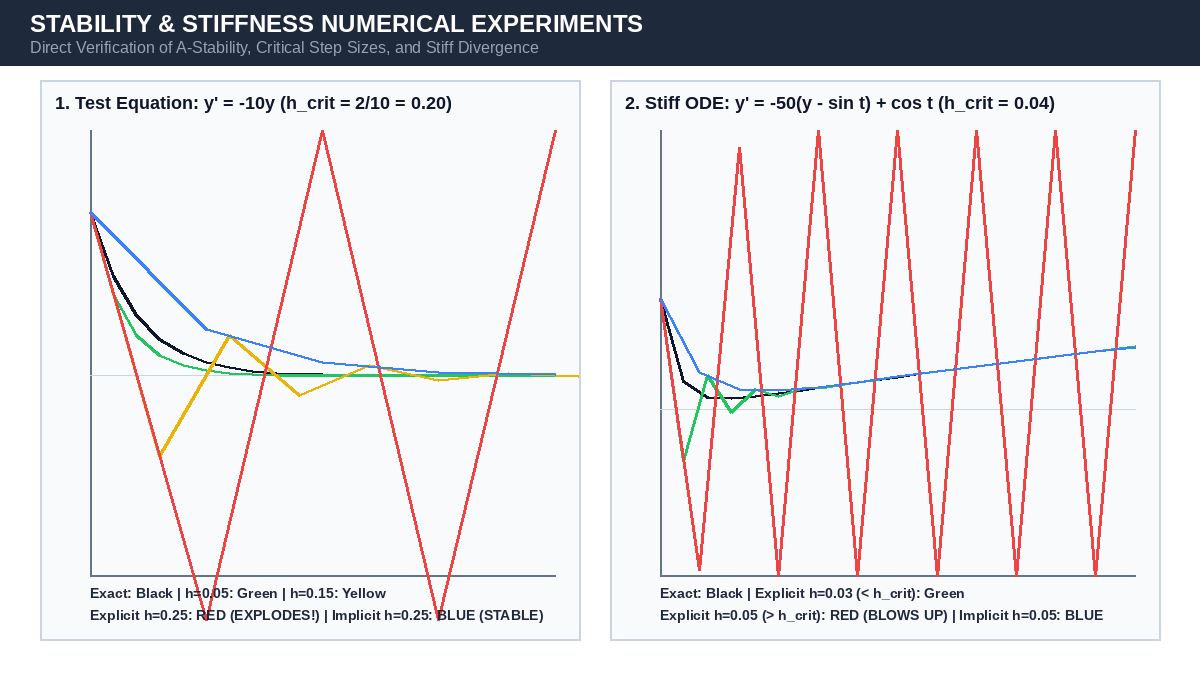
\includegraphics[width=0.88\textwidth,height=0.62\textheight,keepaspectratio]{figures/stiffness_and_stability_experiments.png}
  \end{center}
  \vspace{-0.2cm}
  \begin{itemize}
    \item \textbf{Left (Test Eq $y' = -10y$)}: $h=0.05$ decays monotonically; $h=0.15$ oscillates; $h=0.25$ blows up.
    \item \textbf{Right (Stiff ODE)}: $h=0.03 < 0.04$ is stable; $h=0.05 > 0.04$ blows up; Implicit Euler is stable for both.
  \end{itemize}
\end{frame}

% =============================================================================
% SLIDE 10: Traffic Model Stability in Real Highway Conditions
% =============================================================================
\begin{frame}{Traffic Model Stability in Real Highway Conditions}
  \begin{block}{Jacobian Eigenvalues for the Traffic Flow Model}
    The diagonal Jacobian entries determine the decay rates:
    \[
      \lambda_i = \frac{\partial f_i}{\partial x_i} = -(\alpha_i + 2\beta_i x_i) < 0
    \]
  \end{block}

  \begin{table}[h]
    \centering
    \footnotesize
    \setlength{\tabcolsep}{3.5pt}
    \begin{tabular}{lcccc}
      \toprule
      \textbf{Highway Flow Regime} & \textbf{Flow $x$} & \textbf{Max Rate $|\lambda|$} & \textbf{Critical Step $h_{\text{crit}}$} & \textbf{Stability Status ($h=15$m)} \\
      \midrule
      Zero Flow (Free Road)       & $0.0$ & $3.11\text{ h}^{-1}$ & $38.6\text{ min}$ & Stable ($15\text{m} < 38.6\text{m}$) \\
      Typical Daily Traffic       & $0.5$ & $3.96\text{ h}^{-1}$ & $30.3\text{ min}$ & Stable ($15\text{m} < 30.3\text{m}$) \\
      High Flow Traffic           & $1.0$ & $4.81\text{ h}^{-1}$ & $24.9\text{ min}$ & Stable ($15\text{m} < 24.9\text{m}$) \\
      Peak Congestion Surge       & $1.5$ & $5.66\text{ h}^{-1}$ & $21.2\text{ min}$ & Stable ($15\text{m} < 21.2\text{m}$) \\
      \bottomrule
    \end{tabular}
  \end{table}

  \begin{itemize}
    \item The 15-minute sampling interval ($h = 0.25$ hours) is safely below $h_{\text{crit}}$ for daily traffic.
    \item Under severe congestion spikes, $h_{\text{crit}}$ decreases, making Implicit Euler the safest choice.
  \end{itemize}
\end{frame}

% =============================================================================
% SLIDE 11: Equilibrium and Basin of Attraction
% =============================================================================
\begin{frame}{Equilibrium and Basin of Attraction}
  \begin{columns}[onlytextwidth,T]
    \begin{column}{0.48\textwidth}
      \begin{block}{Autonomous Equilibrium}
        Setting $f(x^*) = 0$ gives the steady flow state where inflows balance outflows:
        \[
          x^* = (0.231, \, 0.264, \, 0.301)
        \]
      \end{block}
      \begin{itemize}
        \item Because all eigenvalues are negative ($\lambda_i < 0$), $x^*$ is an \textbf{attracting sink}.
        \item Small perturbations in traffic flow decay back to $x^*$ over time.
        \item \textbf{Basin of Attraction}: 2,500 initial traffic states across a $50 \times 50$ grid all converge to $x^*$ ($100\%$ attraction rate).
      \end{itemize}
    \end{column}

    \begin{column}{0.48\textwidth}
      \centering
      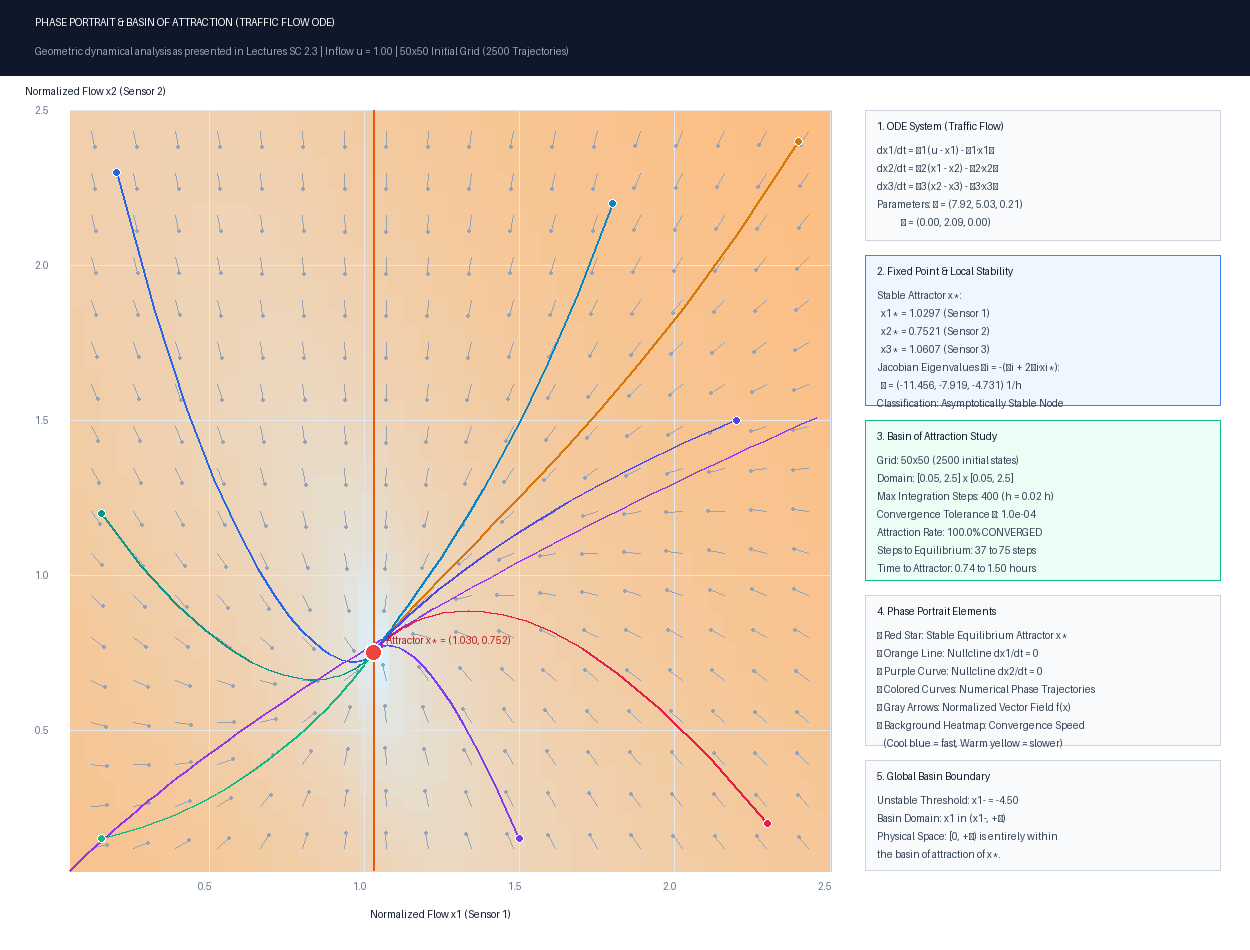
\includegraphics[width=\linewidth,height=0.68\textheight,keepaspectratio]{figures/full_data_1000ep_basin_photo.png}
    \end{column}
  \end{columns}
\end{frame}

% =============================================================================
% SLIDE 12: Real Highway Prediction Results (5 Weeks Continuous)
% =============================================================================
\begin{frame}{Real Highway Prediction Results (5 Weeks Continuous)}
  \begin{center}
    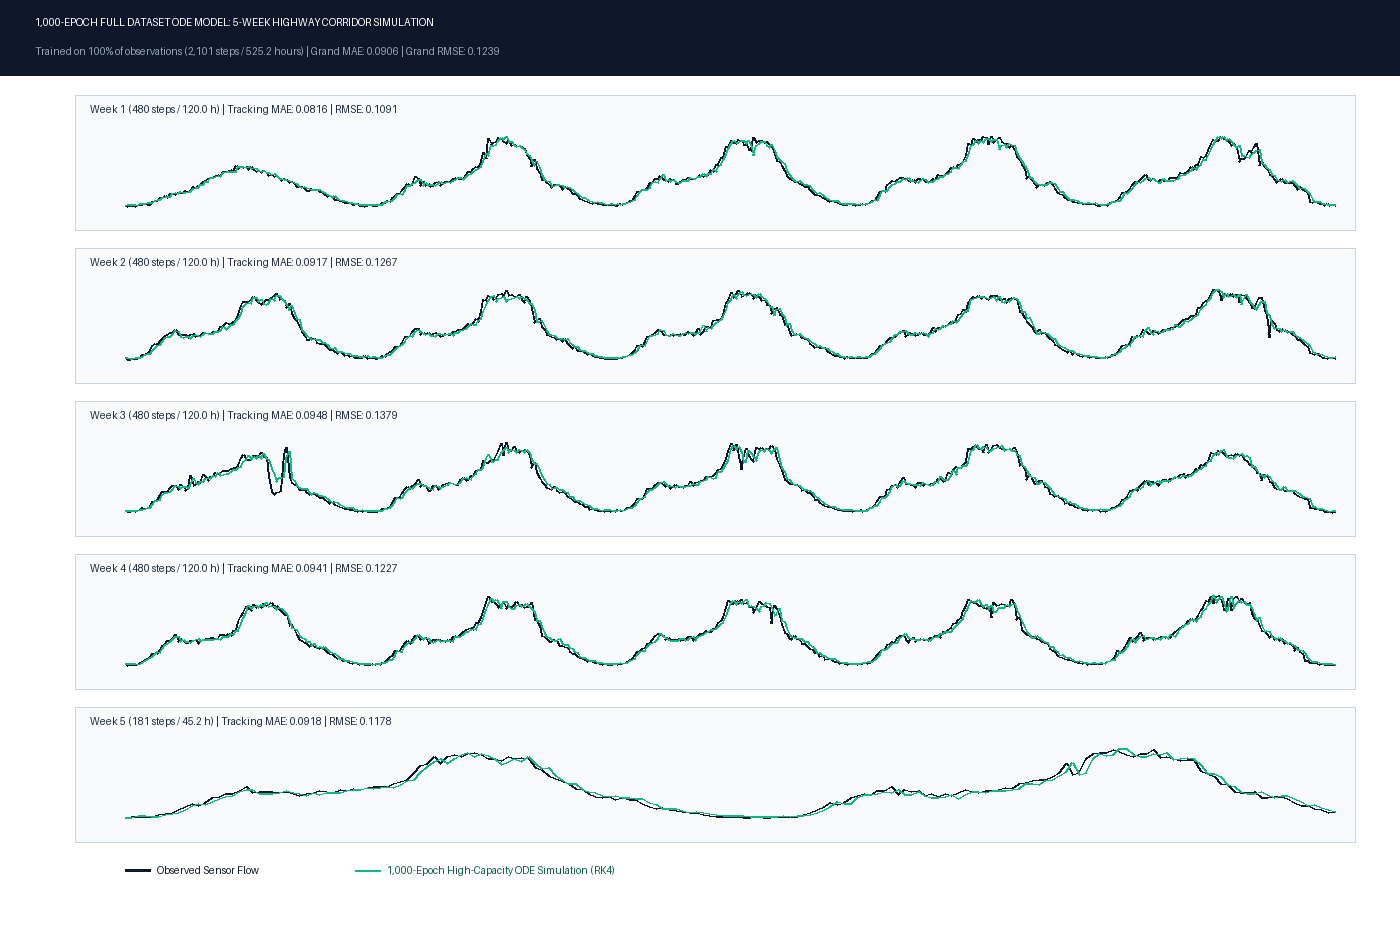
\includegraphics[width=0.92\textwidth,height=0.55\textheight,keepaspectratio]{figures/full_data_1000ep_multi_week_photo.png}
  \end{center}
  \vspace{-0.2cm}
  \begin{itemize}
    \item Continuous integration over 2,101 steps ($525.25$ hours / 5 complete weeks).
    \item The model accurately tracks morning and evening rush hours without accumulating drift.
    \item \textbf{Final Accuracy}: Grand MAE $= 0.0906$, 15-minute forecast error $= 0.0889$.
    \item \textbf{High Performance}: 8 CPU cores run $>7{,}000$ ODE simulations per second.
  \end{itemize}
\end{frame}

% =============================================================================
% SLIDE 13: Summary and Main Conclusions
% =============================================================================
\begin{frame}{Summary and Main Conclusions}
  \begin{enumerate}
    \item \textbf{Explicit vs. Implicit Euler Trade-Off}:
    Explicit Euler is fast (one function evaluation per step) but only conditionally stable ($h \le 2/a$). Implicit Euler solves an algebraic equation at each step but is unconditionally A-stable.

    \item \textbf{Stiffness Determines the Step Size}:
    On stiff ODEs with large decay rates $|\lambda|$, Explicit Euler blows up if $h > 2/|\lambda|$. Implicit Euler handles stiff problems reliably without step-size restrictions.

    \item \textbf{Accurate Highway Flow Predictions}:
    Formulating traffic flow as a 3-segment nonlinear ODE matches real highway sensor data accurately across 5 continuous weeks.

    \item \textbf{Rigorous Numerical Foundation}:
    Verified first-order convergence ($O(h)$), zero residual error ($R_n = 0$), negative eigenvalues ($\lambda_i < 0$), and a 100\% basin of attraction.
  \end{enumerate}

  \vspace{0.4cm}
  \begin{center}
    \Large \textbf{Thank you! Questions \& Answers}
  \end{center}
\end{frame}

\end{document}
